% \title{Apunte de Matemáticas Discretas CC3101:\\ 
% Funciones Generadoras (Parte 2)  Clase 16}
% % \title{Ejercicios Lógica e Inducción}
% \author{Andrés Abeliuk}
% \date{}
% \maketitle


\section{Más sobre funciones generadoras}

\subsection{Coeficientes Binomiales}
Las funciones generadoras no solo sirven para encontrar soluciones cerradas a recurrencias, sino que también son \emph{herramientas poderosas para resolver problemas de conteo sofisticados}. Para esto, necesitamos extender la noción de coeficientes binomiales a casos más generales.

A continuación definimos los coeficientes binomiales extendidos, los cuales permiten trabajar con exponentes reales y negativos en funciones generadoras.

\begin{definitionblock}{Coeficiente Binomial Extendido}
Sea $r$ cualquier número real y $k$ un entero. Se define:
$$
  \binom{r}{k} =
  \begin{cases}
    \dfrac{r(r-1)\cdots (r-k+1)}{k!} & \text{si } k \geq 0, \\
    0 & \text{si } k < 0.
  \end{cases}
$$
\end{definitionblock}

\subsubsection*{Ejemplos:}
Veamos algunos ejemplos ilustrativos del uso de esta definicion en casos no enteros o negativos.
\begin{itemize}
\item $\displaystyle \binom{-2}{3} = \frac{-2 \cdot -3 \cdot -4}{3!} = -4$
\item $\displaystyle \binom{1/2}{3} = \frac{1/2 \cdot (-1/2) \cdot (-3/2)}{6} = 1/16$
\end{itemize}

Finalmente, resumimos algunas propiedades algebraicas importantes de estos coeficientes.
\begin{thmblock}{Propiedades de los Coeficientes Binomiales}
\begin{itemize}

\item $\displaystyle
  \binom{-r}{k} = (-1)^k \binom{r + k - 1}{k}$, si  $k,r\geq 0$.

\item $\displaystyle \binom{r}{k} = \frac{r}{k} \binom{r-1}{k-1}$, si $k \neq 0$.
\item Identidad de simetría: $\displaystyle \binom{r}{k} = \binom{r}{r-k}$, si $r, k$ son enteros con $r \geq 0$.
\end{itemize}
\end{thmblock}

\subsection{Teorema del Binomio Extendido}
El siguiente resultado extiende el teorema binomial a exponentes reales.
\begin{thmblock}{Teorema del Binomio Extendido}
Sea $r \in \mathbb{R}$ y $x,y$ reales tales que $|x/y|<1$, entonces:

$$
(x+y)^r = \sum_{k=0}^{\infty} \binom{r}{k} x^k y^{r-k}.
$$

\end{thmblock}
Notar que, si $r$ es un entero no negativo, entonces $\binom{r}{k} = 0$ para todo $k > r$, por lo que la serie se reduce a una suma finita.  Esto se debe a que el numerador del coeficiente binomial incluye un término nulo al multiplicar más allá de \( r \). Por ejemplo, el término \( (r - k + 1) \) será cero o negativo si \( k > r \), lo que hace que el producto total se anule y, por tanto, \( \binom{r}{k} = 0 \).
     
En cambio, si $r$ no es un entero no negativo, la serie es infinita y requiere condiciones de convergencia, como que $|x/y|<1$. Intuitivamente, cuando \( x \) es suficientemente pequeño en relación a \( y \), los términos de la serie se atenúan y la suma infinita converge. 
% Si \( |x/y| \geq 1 \), la serie puede divergir dependiendo del valor de \( r \), por lo que esta restricción es necesaria para garantizar que el desarrollo sea válido.


Un caso especial ocurre cuando $y = 1$, obteniendo:
$$(1+x)^r = \sum_{k=0}^{\infty} \binom{r}{k} x^k.$$


% \subsection{Aplicación: funciones generadoras}
% Veamos ahora algunas funciones generadoras comunes y las sucesiones que generan.

% \begin{exampleblock}{Función generadora de $(1+x)^{-n}$}

% $$
%   (1+x)^{-n} = \sum_{k=0}^{\infty} (-1)^k \binom{n+k-1}{k} x^k.
% $$

% Genera la sucesión $\langle (-1)^k \binom{n+k-1}{k} \rangle\_{k \geq 0}$.
% \end{exampleblock}

% \begin{exampleblock}{Función generadora de $(1-x)^{-n}$}

% $$
%   (1-x)^{-n} = \sum_{k=0}^{\infty} \binom{n+k-1}{k} x^k.
% $$

% Genera la sucesion $\langle \binom{n+k-1}{k} \rangle\_{k \geq 0}$.
% \end{exampleblock}

\subsection{Aplicación: Números de Catalán}

Los números de Catalán surgen en una gran variedad de contextos combinatorios. Uno de los ejemplos clásicos es el cómputo del número de \emph{árboles binarios diferentes con $n$ vértices}. A continuación desarrollamos la función generadora de los números de Catalán paso a paso, partiendo desde su definición recursiva.


\begin{exampleblock}{Ejemplo: \textbf{Árboles binarios}}
\begin{center}
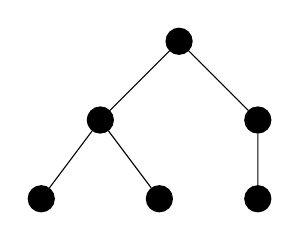
\begin{tikzpicture}[
every node/.style={circle, draw, fill=black,minimum size=2mm},
level 1/.style={sibling distance=20mm},
level 2/.style={sibling distance=15mm},
level 3/.style={sibling distance=7.5mm},
level distance=10mm
]
\node {}
child {node {}child {node {}}
child {node {}}}
child {node {}child {node {}}
};
\end{tikzpicture}
\end{center}
Para contar los árboles binarios con $n$ vértices, comenzamos con un nodo raíz y distribuimos los restantes $n-1$ nodos entre el subárbol izquierdo (con $k$ vértices) y el derecho (con $n-1-k$ vértices). Esto produce la recurrencia:
$$
C_n = \sum_{k=0}^{n-1} C_k C_{n-k-1}, \quad C_0 = 1.
$$
\end{exampleblock}



\begin{exampleblock}{Ejemplo: \textbf{Secuencias de paréntesis balanceados}}
Otra interpretación clásica de los números de Catalán es contar cuántas secuencias de paréntesis bien balanceadas existen con $n$ pares de paréntesis. 
Por ejemplo, para $n = 3$ hay exactamente 5 secuencias válidas:
(()()); ()()(); (())(); (()()); ((())).
Esto también se modela con la misma recurrencia de Catalán.
\end{exampleblock}

\begin{thmblock}{Fórmula cerrada de los números de Catalán}
$$
C_n = \frac{1}{n+1} \binom{2n}{n}.
$$
\end{thmblock}
\begin{proof}
Definimos la función generadora:
$$
C(x) = \sum_{n \geq 0} C_n x^n.
$$
Reescribiendo la recurrencia como $C_{n+1} = \sum_{k=0}^{n} C_k C_{n-k}$, y multiplicando ambos lados por $x^n$ y sumando:
$$
\sum_{n \geq 0} C_{n+1} x^n = \sum_{n \geq 0} \left( \sum_{k=0}^{n} C_k C_{n-k} \right) x^n.
$$
 Al lado derecho, obtenemos la convolución resultante de multiplicar $C(x)$ por sí misma:
\begin{align*}
   \sum_{n=0}^{\infty}\left(\sum_{k=0}^{n}C_kC_{n-k}\right) x^n &~=~ 
   \left(\sum_{n\geq 0}{C_nx^n}\right)^2 ~=~ C^2(x)
\end{align*}  
El lado izquierdo es $\frac{1}{x}(C(x) - 1)$, por lo tanto:
$$
\frac{1}{x}(C(x) - 1) = C(x)^2 \quad \Rightarrow \quad xC(x)^2 - C(x) + 1 = 0.
$$
Resolvemos la ecuación cuadrática:
$$
C(x) = \frac{1 \pm \sqrt{1 - 4x}}{2x}.
$$
¿cuál raíz es la correcta? 
Seleccionamos la raíz negativa ya que debe cumplirse $C(0) = \sum_{n \geq 0} C_n 0^n =C_0 = 1$, y la otra opción diverge. Obtenemos:
$$
C(x) = \frac{1 - \sqrt{1 - 4x}}{2x}.
$$
\textbf{Aplicando el teorema del binomio extendido} a $\sqrt{1 - 4x}$, derivamos la serie de potencias:
$$
\sqrt{1 - 4x} = \sum_{n = 0}^{\infty} (-4)^n \binom{1/2}{n} x^n. 
$$
% Tras manipular algebraicamente esta expresión, obtenemos finalmente:
% $$
% C_n = \frac{1}{n+1} \binom{2n}{n}.
% $$
Cambiando el indice inicial de la serie de potencia, dado que $\binom{1/2}{0}=1$ , obtenemos:
$$
1 - \sqrt{1 - 4x} =1- \left(\sum_{n = 1}^{\infty} (-4)^n \binom{1/2}{n} x^n + 1\right) = \sum_{n = 1}^{\infty} (-4)^{n} \binom{1/2}{n} x^n
$$
Con eso obtenemos 
\begin{align*}    
C(x) &~=~ \frac{1}{2x}(1-\sqrt{1 - 4x})
=\frac{1}{2x}\sum_{n = 1}^{\infty} (-4)^{n} \binom{1/2}{n} x^n\\
&~=~ \frac{1}{2}\sum_{n = 1}^{\infty} (-4)^{n} \binom{1/2}{n} x^{n-1}
=\frac{1}{2}\sum_{n = 0}^{\infty} (-4)^{n+1} \binom{1/2}{n+1} x^{n}
\end{align*} 
Por lo tanto, 
$$
C_n =  \frac{1}{2}(-4)^{n+1} \binom{1/2}{n+1} 
$$
\textbf{~Simplificación del coeficiente.}  
  \begin{align*}
      \binom{0.5}{n}(-4)^n &~=~ \frac{0.5(0.5-1)\cdots (0.5-n+1)}{n!}\cdot (-4)^n
       ~=~ \frac{2(2-4)\cdots (2-4n+4)}{n!}(-1)^n\\
      & ~=~ -\frac{2(2)(6)\cdots (4n-6)}{n!}
      ~=~ -\frac{2^n(1)(3)\cdots (2n-3)}{n!}\\
      &  ~=~ -\frac{(n!\cdot 2^n)\cdot (1)(3)\cdots (2n-3)}{n!n!}
     ~=~ -\frac{(2n)!}{n!n!(2n-1)}\\
        & ~=~ - \frac{1}{2n-1}\binom{2n}{n}
    \end{align*} 
Por lo tanto,
$$
C_n = \frac{1}{2}(-4)^{n+1} \binom{1/2}{n+1}  = \frac{1}{2(n+2)} \binom{2(n+1)}{n+1} = \frac{1}{n+1} \binom{2n}{n}.
$$
\end{proof}


\subsection{Problemas de Conteo y Funciones Generadoras}

\begin{exampleblock}{Ejemplo: suma con restricciones}
¿Cuántas soluciones existen de $e_1 + e_2 = 8$ sujeto a:
$\left\{\begin{array}{l} 2\leq e_1\leq 5,\\ 3\leq e_2\leq 6\end{array}\right.$?

Construimos los polinomios generadores asociados a los posibles valores de $e_1$ y $e_2$:

\[
f_1(x) = x^2 + x^3 + x^4 + x^5, \quad f_2(x) = x^3 + x^4 + x^5 + x^6.
\]

El producto $f_1(x) \cdot f_2(x)$ representa todas las combinaciones posibles de $e_1$ y $e_2$, y el coeficiente de $x^8$ en su expansión indica cuántas sumas satisfacen $e_1 + e_2 = 8$ bajo las restricciones dadas.
$$
f_1(x) f_2(x) = x^5 + 2x^6 + 3x^7 + \textcolor{red}{4x^8} + 3x^9 + 2x^{10} + x^{11}.
$$
Por lo tanto, hay \textbf{4 maneras} de formar $x^8$, combinando exponentes del primer polinomio con los del segundo de modo que sus sumas den $8$. Las combinaciones que generan este término son:
\[
\textcolor{red}{2+6}, \quad \textcolor{red}{3+5}, \quad \textcolor{red}{4+4}, \quad \textcolor{red}{5+3}.
\]
\end{exampleblock}

\begin{exampleblock}{Ejemplo: suma generalizada}
¿Cuántas soluciones existen de $e_1 + e_2 + e_3 = 14$ sujeto a:
$\left\{\begin{array}{l} 2\leq e_1\leq 5,\\ 3\leq e_2\leq 6\\
  4\leq e_3\leq 7\end{array}\right.$?

Usamos:

$$
f(x) = (x^2 + x^3 + x^4 + x^5)(x^3 + x^4 + x^5 + x^6)(x^4 + x^5 + x^6 + x^7).
$$

El número de soluciones es el coeficiente de $x^{14}$ en $f(x)$. Esto se debe a que al multiplicar los tres polinomios, el término $x^i x^j x^k$ aparece en el producto cuando $i + j + k = 14$, es decir, cuando las elecciones de $e_1$, $e_2$ y $e_3$ suman 14.

% \textbf{Moraleja:} Sea $f(x) = \sum_{n \geq 0} a_n x^n$ el polinomio resultante. Entonces $a_{14}$ nos da directamente la cantidad de soluciones al problema original.

\end{exampleblock}

\begin{exampleblock}{Ejemplo: Distribución de objetos con cotas}
¿De cuántas maneras se pueden distribuir 8 galletas idénticas entre 3 perritos distintos, si cada uno recibe entre 2 y 4 galletas?

Las posibilidades para cada perrito son $2\leq p_i\leq 4$, y pueden capturarse en $3$ exponentes: $(x^2+x^3+x^4)$

Todas las combinaciones de $3$ perritos se capturan con la \textbf{funci\'on generadora}:
$$
G(x) = (x^2 + x^3 + x^4)^3.
$$
Expandiendo:
$$
G(x) = x^{12} + 3x^{11} + 6x^{10} + 7x^9 + \boxed{6x^8} + 3x^7 + x^6.
$$
La respuesta est\'a en el coeficiente de $x^8$, esto es, $6$. 
\end{exampleblock}


% \subsection*{Formas de pagar con monedas}

\newcommand{\circledone}{\textcolor{blue}{\raisebox{.5pt}{\textcircled{\raisebox{-.9pt} {\small 1}}}}}
\newcommand{\circledtwo}{\textcolor{red}{\raisebox{.5pt}{\textcircled{\raisebox{-.9pt} {\small 2}}}}}
\newcommand{\circledfive}{\textcolor{green!60!black}{\raisebox{.5pt}{\textcircled{\raisebox{-.9pt} {\small 5}}}}}

\begin{exampleblock}{Formas de pagar con monedas}

Supongamos que tenemos monedas de 1 euro, 2 euros, y 5 euros (representadas por $\circledone$, $\circledtwo$, y $\circledfive$ respectivamente), y queremos contar todas las \textcolor{red}{maneras de pagar un total de $r$ euros} en una máquina.

Considere dos casos: cuando el orden \textbf{sí importa} y cuando el orden \textbf{no importa}.

\medskip
\textbf{Ejemplo:} si $r = 5$, entonces:

\begin{minipage}{0.6\textwidth}
\underline{\textbf{Orden SÍ importa:}}

\begin{enumerate}
  \item $5 \times \circledone$: 1 forma: \quad $\circledone\circledone\circledone\circledone\circledone$
  \item $3 \times \circledone$ + $\circledtwo$: 4 formas:
  \[
  \circledone\circledone\circledone\circledtwo,\quad
  \circledone\circledone\circledtwo\circledone,\quad
  \circledone\circledtwo\circledone\circledone,\quad
  \circledtwo\circledone\circledone\circledone
  \]
  \item $1 \times \circledone$ + $2 \times \circledtwo$: 3 formas:
  \[
  \circledone\circledtwo\circledtwo,\quad
  \circledtwo\circledone\circledtwo,\quad
  \circledtwo\circledtwo\circledone
  \]
  \item $\circledfive$: 1 forma.
\end{enumerate}

\textbf{Total:} 9 maneras
\end{minipage}%
\hfill
\begin{minipage}{0.35\textwidth}
\underline{\textbf{Orden NO importa:}}

\begin{enumerate}
  \item $5 \times \circledone$
  \item $3 \times \circledone$ + $\circledtwo$
  \item $\circledone$ + $2 \times \circledtwo$
  \item $\circledfive$
\end{enumerate}

\textbf{Total:} 4 maneras
\end{minipage}

\end{exampleblock}

\subsubsection*{Solución: Formas de pagar con monedas (caso orden no importa)}
Este problema se modela usando una función generadora infinita, en la cual consideramos que podemos usar cualquier cantidad (incluyendo cero) de cada tipo de moneda:

\[
F(x) = \underbrace{(1 + x + x^2 + x^3 + \dots)}_{\text{monedas de 1 euro}} 
\cdot \underbrace{(1 + x^2 + x^4 + x^6 + \dots)}_{\text{monedas de 2 euros}} 
\cdot \underbrace{(1 + x^5 + x^{10} + x^{15} + \dots)}_{\text{monedas de 5 euros}}.
\]

Este producto genera un término $x^r$ por cada forma de sumar exactamente $r$ euros con las monedas disponibles, sin importar el orden.
Esto, porque cada combinación de monedas genera un producto $x^{i + 2j + 5k}$, donde $i$, $j$, y $k$ son la cantidad de monedas de 1, 2 y 5 euros, respectivamente. El coeficiente de $x^r$ en $F(x)$ cuenta cuántas combinaciones de este tipo suman $r=5$.

% \end{exampleblock}

% \begin{exampleblock}{Ejemplo concreto con $r = 5$}

Podemos calcular el coeficiente de \(x^r\) descomponiendo la función generadora en fracciones parciales, multiplicando manualmente los polinomios, o utilizando herramientas computacionales como \texttt{Matlab} o \texttt{Wolfram Alpha}.

% Para calcular cuántas maneras hay de pagar 5 euros, evaluamos el coeficiente de $x^5$ en la expansión:
\[
F(x) = \frac{1}{(1 - x)(1 - x^2)(1 - x^5)}.
\]
\noindent Su expansión comienza como:
\[
F(x) = 1 + x + 2x^2 + 2x^3 + 3x^4 + \boxed{4x^5} + 5x^6 + 6x^7 + \dots
\]
Por lo tanto, hay \textbf{4 maneras} de pagar 5 euros con monedas de 1, 2 y 5 euros si el orden no importa.

% \end{exampleblock}


\subsubsection*{Solución: Formas de pagar con monedas (caso orden SÍ importa)}

% \begin{exampleblock}{Ejemplo con número fijo de monedas}

Supongamos que tenemos monedas de 1, 2 y 5 euros, y queremos pagar un total de $r$ euros usando exactamente $n$ monedas. Cuando el orden \textbf{sí importa}, esto se modela con la función generadora:
$$
G(x) = (x + x^2 + x^5)^n.
$$
El coeficiente de $x^r$ en este polinomio cuenta las maneras distintas de elegir $n$ monedas (considerando el orden) cuya suma sea $r$.

% \medskip

\begin{exampleblock}{Ejemplo: } 
Si $n = 2$, entonces:
$$
G(x) = (x + x^2 + x^5)^2 = x^2 + 2x^3 + x^4 + 2x^6 + 2x^7 + x^{10}.
$$
El coeficiente de $x^3$ es 2, pues existen dos formas ordenadas de pagar 3 euros con 2 monedas:
$$
\circledone\circledtwo, \quad \circledtwo\circledone.
$$
\end{exampleblock}

% \begin{exampleblock}{Caso general: número variable de monedas}
\medskip

Pero queremos \emph{cualquier n\'umero de monedas} que juntas den $r$ euros, no s\'olo $n$ de ellas, por eso debemos considerar m\'as valores de $n$.
Si se permite cualquier cantidad de monedas, la función generadora total es una suma infinita:
\begin{eqnarray*}
F(x) & = & \sum^\infty_{i=0}(x + x^2 + x^5)^i \\
& = &  \frac{1}{1-(x+x^2+x^5)} ~=~ \frac{1}{1-x-x^2-x^5} 
\end{eqnarray*} 
La expansión comienza como:
$$
F(x) = 1 + x + 2x^2 + 3x^3 + 5x^4 + \boxed{9x^5} + 15x^6 + 26x^7 + 44x^8 + 75x^9 + \dots
$$

Por lo tanto, hay \textbf{9 maneras} de pagar 5 euros con monedas de 1, 2 y 5 euros si el orden sí importa y se pueden usar tantas monedas como se desee.

% \end{exampleblock}





\subsection*{Ejercicios propuestos}
\begin{itemize}
\item ¿De cuántas maneras se pueden entregar 12 peluches idénticos a 5 niños, si cada uno recibe a lo más 3 peluches?
\item ¿Cuántas maneras hay de pagar 8 euros con monedas de 1, 2, 3, y 4 euros si el orden \textbf{no importa}?
\item ¿Y si el orden \textbf{sí importa} para pagar 7 euros con las mismas monedas?
\end{itemize}



 % \subsection*{Referencias}
 %   \begin{itemize}
 %     \item ``Concrete Mathematics'' de R.~Graham, D.~Knuth, y O.~Patashnik, 2da.\ edici\'on, Addison-Wesley, 1994. 
 %    \item ``Generatingfunctionology'', de Herbert S. Wilf. Disponible en 
 %    \url{https://www.math.upenn.edu/~wilf/DownldGF.html}, 1994.
 %   \end{itemize} 
  